% !TeX spellcheck = it_IT 
\documentclass[11pt]{article}
\usepackage[italian]{babel}
\usepackage[T1]{fontenc}
\usepackage[utf8]{inputenc}
\usepackage{graphicx}
\usepackage{todonotes}
\usepackage{listings}
\usepackage{caption}
\usepackage{subcaption}
\usepackage{abbrevs}



\definecolor{dkgreen}{rgb}{0,0.6,0}
\definecolor{gray}{rgb}{0.5,0.5,0.5}
\definecolor{mauve}{rgb}{0.58,0,0.82}

\lstset{
  frame=single,
  captionpos=b,
  language=Java,
  aboveskip=3mm,
  belowskip=3mm,
  showstringspaces=false,
  columns=flexible,
  basicstyle={\small\ttfamily},
  numbers=none,
  numberstyle=\tiny\color{gray},
  keywordstyle=\color{blue},
  commentstyle=\color{dkgreen},
  stringstyle=\color{mauve},
  breaklines=true,
  breakatwhitespace=true,
  tabsize=3
}

\makeatletter
\def\cleardoublepage{
	\clearpage\if@twoside \ifodd\c@page\else
	\hbox{}
	\thispagestyle{empty}
	\newpage
	\if@twocolumn\hbox{}\newpage\fi\fi\fi
}

\makeatother

\setlength{\textwidth}{14cm}
\setlength{\textheight}{21cm}
\setlength{\footskip}{3cm}

\setlength{\hoffset}{0pt}
\setlength{\voffset}{0pt}

\setlength{\oddsidemargin}{1cm}
\setlength{\evensidemargin}{1cm}

\begin{document}
	\title{ROVIS - ROver for VIdeo Streaming\large\\Corso di Fisica dei Sistemi Complessi - Prof. Sandro Rambaldi}

	
	\author{Alessandro Cordella \\Natale Vadalà\\alessandro.cordella@studio.unibo.it\\natale.vadala@studio.unibo.it}\large
	\date{Novembre 2018}
	\maketitle
	\newpage
	\tableofcontents
	\newpage
\section{Introduzione}
L'obiettivo del presente lavoro è stato quello di costruire un robot capace di muoversi su ruote e trasmettere un canale di \textit{streaming video over HTTP}. Il dispositivo ottenuto è controllabile da un'interfaccia web ed è possibile visionare ciò che è posto di fronte al robot tramite una webcam.\\Nelle seguenti sezioni verranno descritte le fasi di progettazione e realizzazione, i componenti hardware e le tecniche software utilizzate, e verranno presentati eventuali sviluppi futuri.
\section{Progettazione}
La fase di progettazione è stata condotta attraverso l'analisa della specifica e lo studio di progetti open-source precedenti.
\subsection{Specifica}
Progettare e realizzare un robot, controllabile attraverso un'interfaccia Web, dotato di una webcam in modo da poter trasmettere lo streaming video sulla stessa interfaccia.\\
Inoltre, si richiede l'uso microcontrollore o di un single-board computer, di componenti low-cost e software open-source.
\subsection{Analisi dei requisiti}
\paragraph{Hardware}
Ciò che serve per realizzare ROVIS:
\begin{itemize}
\item \underline{Microcontrollore / Single-board computer}\\
Si è deciso di utilizzare un RaspberryPi 3 model B\footnote{https://www.raspberrypi.org/products/raspberry-pi-3-model-b/}, che presenta nativamente una scheda di rete wireless, sebbene vada bene un qualsiasi Raspberry dotato di scheda di rete (interna o esterna) e porta USB per la webcam.
\item \underline{Una "carrozzeria" con tutti gli alloggi necessari e 4 motori continui}\\
Per semplicità si è deciso di acquistare un \textit{case}\footnote{https://www.diymore.cc/collections/robot-chassis/products/diymore-4-wheel-robot-chassis-smart-car-with-speed-and-tacho-encoder-for-arduino-raspberry-pi-robot-diy-kits-65x26mm-tire} che comprendesse già i motori fissati, evitando di incorrere in ulteriori future complicazioni con l'asseblaggio e messa in asse delle ruote, del moto, ecc...\\
\item \underline{Una scheda che faccia da driver per i motori}\\
Acquistata su Amazon.it\footnote{http://amzn.eu/d/a9PD82e}, una shield con dei chip L293D\footnote{https://www.robot-italy.com/it/l293d-motor-driver.html} (driver per motori molto comuni), permette di collegare i motori e gestirne la direzione (moto orario/antiorario)  e la velocità, ottebibili grazie allo sfruttamento di alcuni pin GPio d'appoggio per il controllo singolo di ogni motore ai e ponti H per permettere i cambi di direzione. Va alimentato con 5V.
\item \underline{Un Power-bank e un alloggiamento\\ per per shield e motori} \\
Si è deciso di utilizzare un power bank per il RaspberryPi per il semplice motivo che è più comodo, a nostro avviso, servire l'alimentazione da una porta micro USB invece che saldare un ulteriore alloggiamento per batterie sul RaspberryPi (Ma andrebbe comunque un'alimentazione uguale a quella per i motori e la shield, cioè 4* batterie AAA quindi 4.8-5V).

\end{itemize}

\begin{figure}[htp]
				\centering
		\begin{subfigure}[b]{0.6\textwidth}

		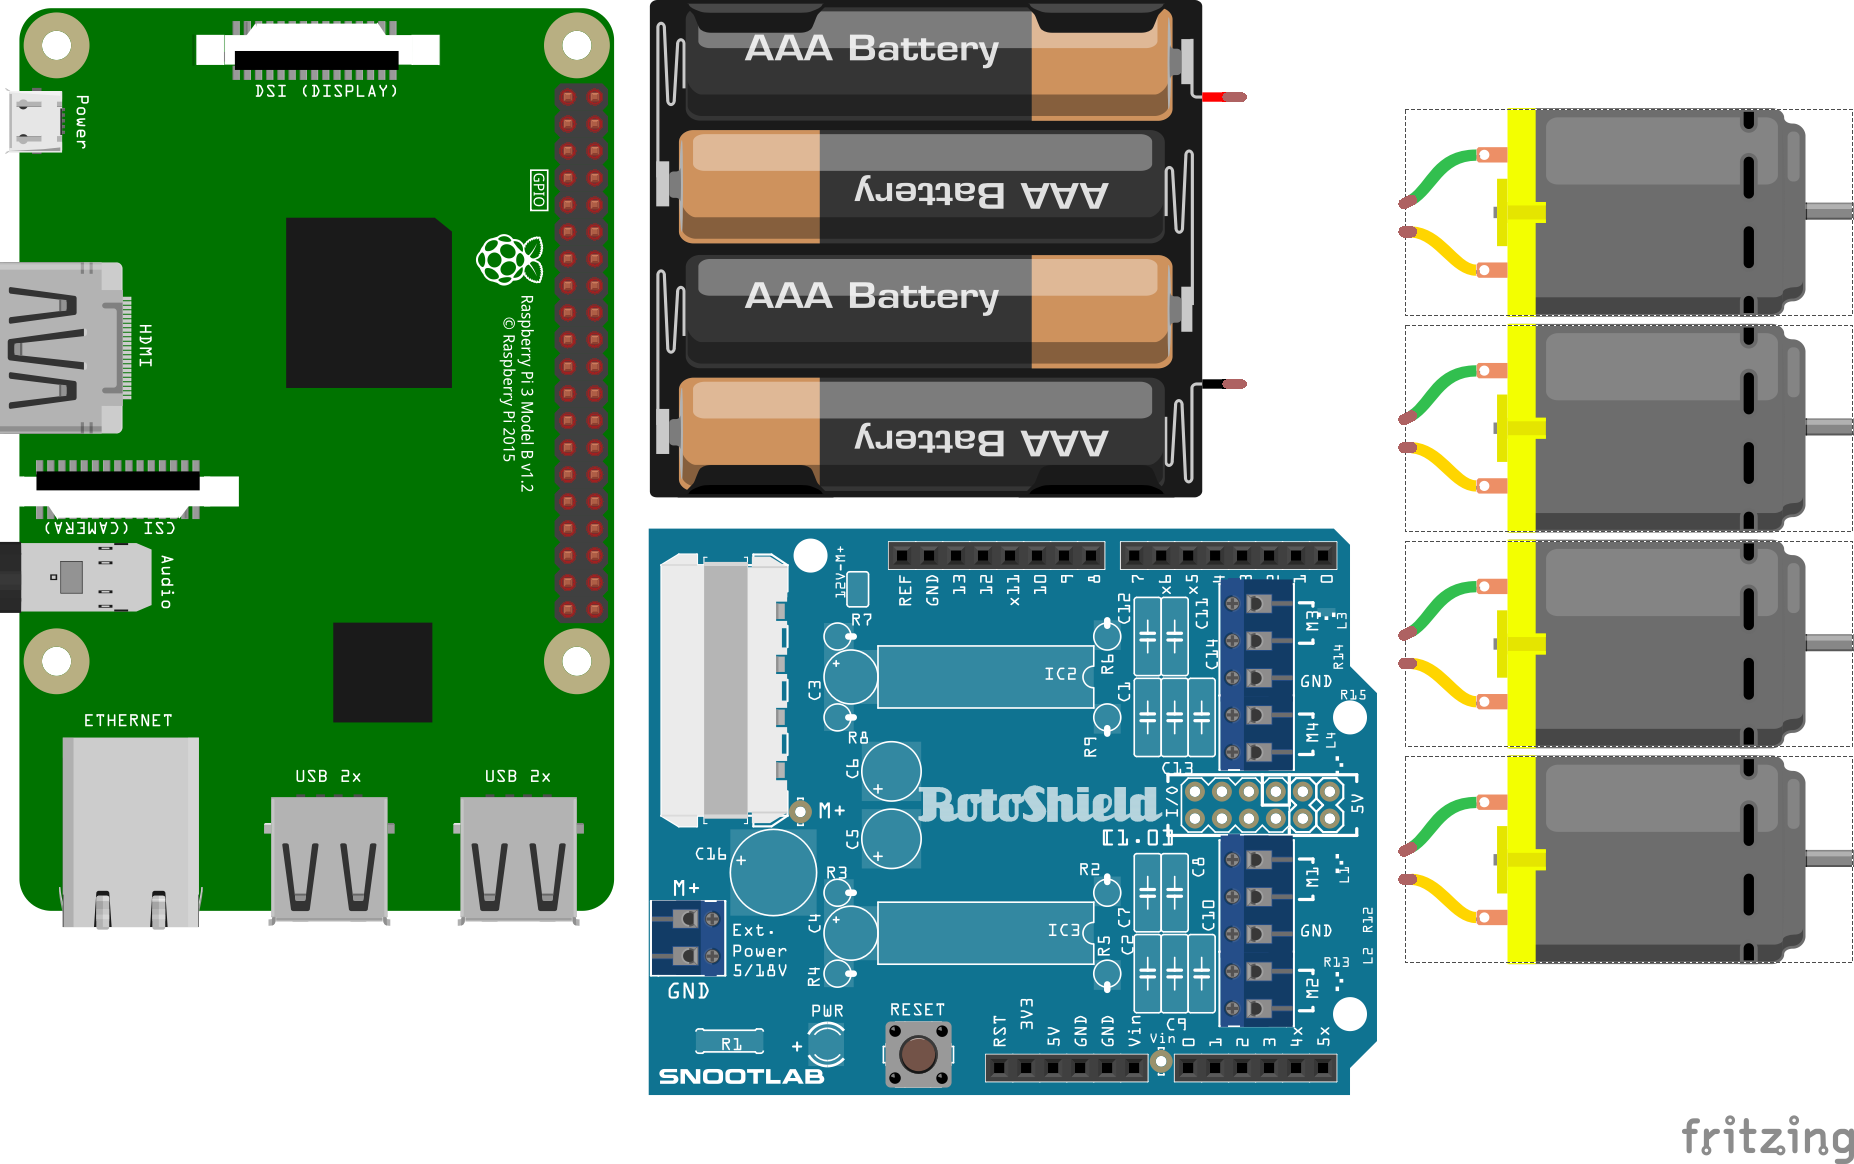
\includegraphics[width=\textwidth]{images/componentsROVIS.png}
		\caption{RaspberryPi, case per batterie, 4 motori continui e L293D drive shield}
		\label{fig:components}
	\end{subfigure}
\\
	%
	\begin{subfigure}[b]{0.4\textwidth}
		
		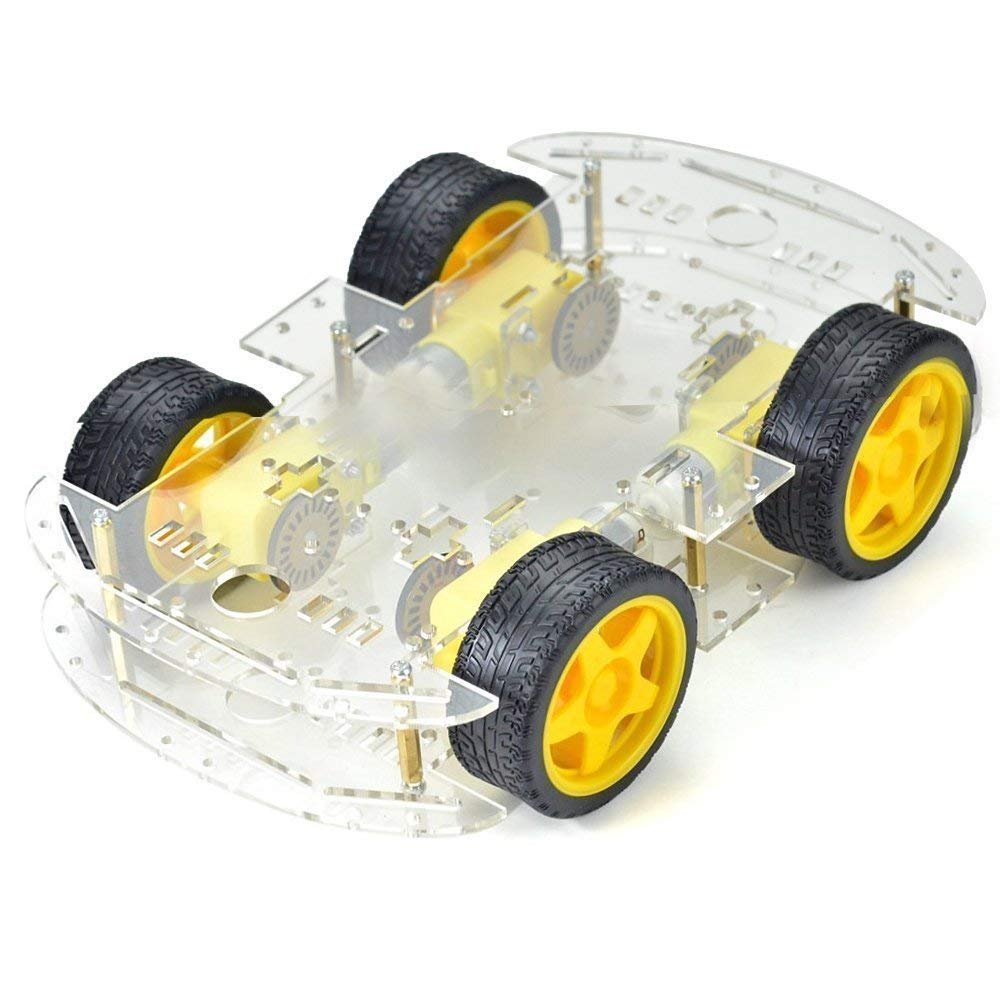
\includegraphics[width=\textwidth]{images/car.jpg}
		\caption{\textit{Case} con motori e ruote}
	\label{fig:car}
	\end{subfigure}
	%
	\begin{subfigure}[b]{0.4\textwidth}
		
		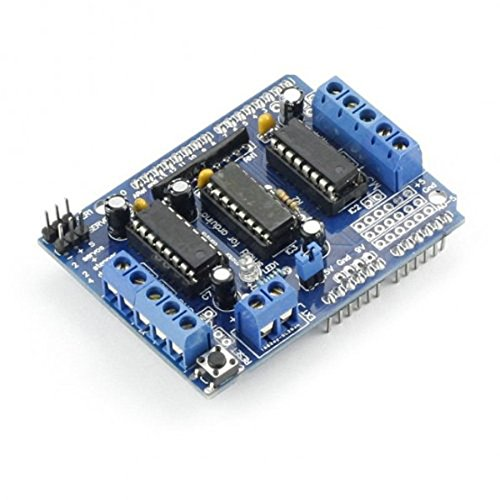
\includegraphics[width=\textwidth]{images/l293d.jpg}
		\caption{L293D drive shield}
	\label{fig:car}
	\end{subfigure}
\end{figure}
\paragraph{Software}
\todo{scrivere un po' di cose, domani sarò fatto}

\begin{figure}[htp]
	\centering
	\begin{subfigure}[b]{0.6\textwidth}
		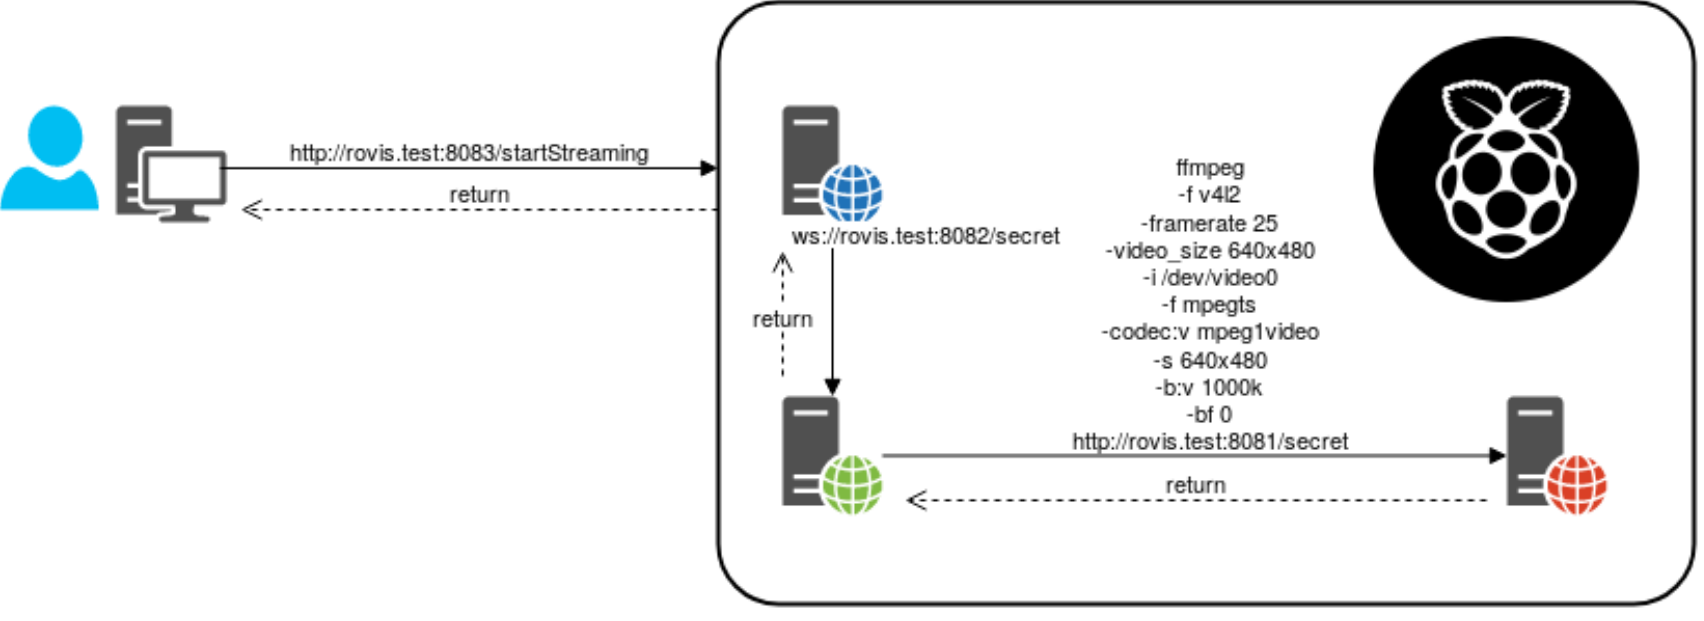
\includegraphics[width=\textwidth]{images/api1.png}
		\caption{Caso d'uso 1: \textbf{\textit{stop streaming}}}
		\label{fig:usecase1}
	\end{subfigure}
	\\
	%
	\begin{subfigure}[b]{0.6\textwidth}	
		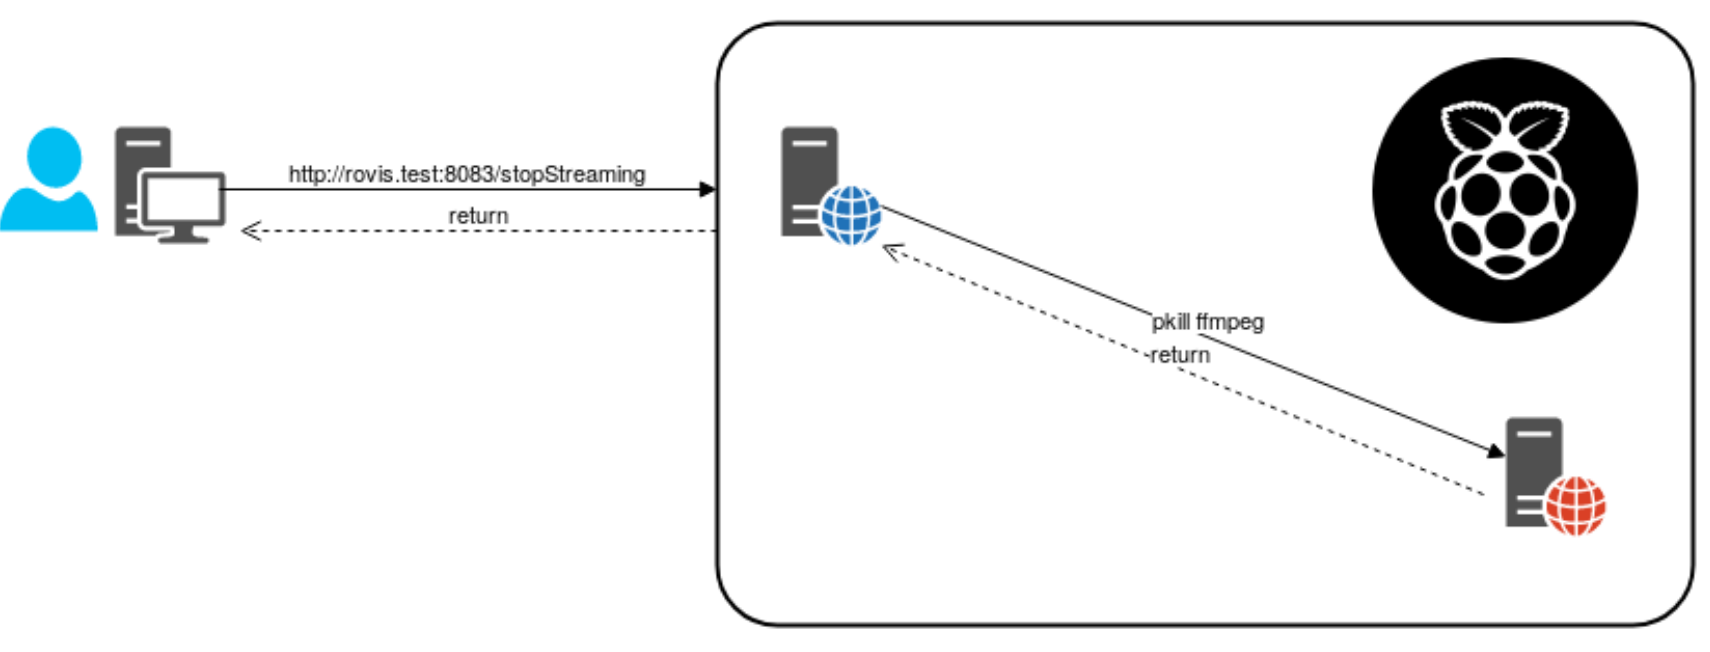
\includegraphics[width=\textwidth]{images/api2.png}
		\caption{Caso d'uso 2: \textbf{\textit{stop streaming}}}
		\label{fig:usecase2}
	\end{subfigure}
	%
	\begin{subfigure}[b]{0.6\textwidth}
		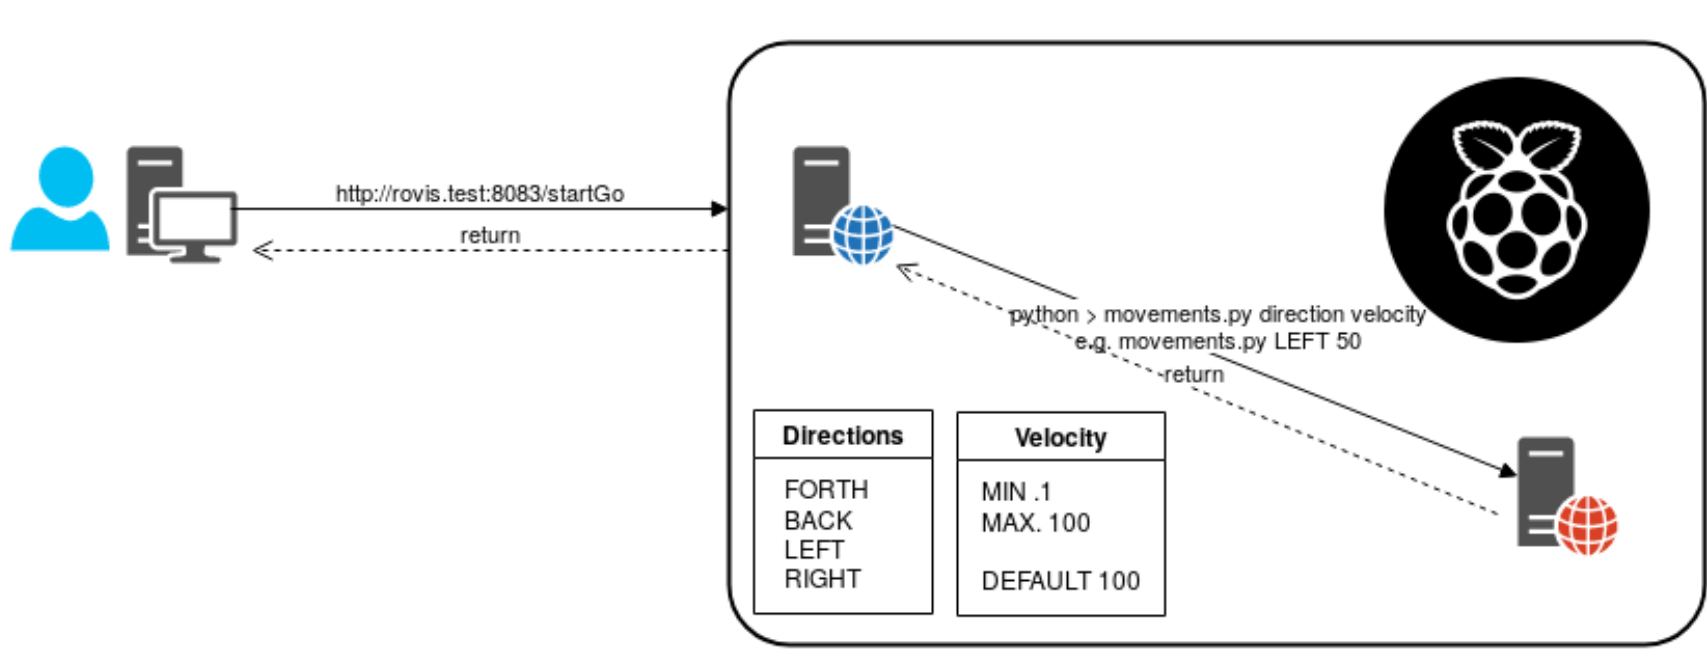
\includegraphics[width=\textwidth]{images/api3.png}
		\caption{Caso d'uso 3: \textbf{\textit{start go}}}
		\label{fig:usecase3}
	\end{subfigure}
	\begin{subfigure}[b]{0.6\textwidth}
	
		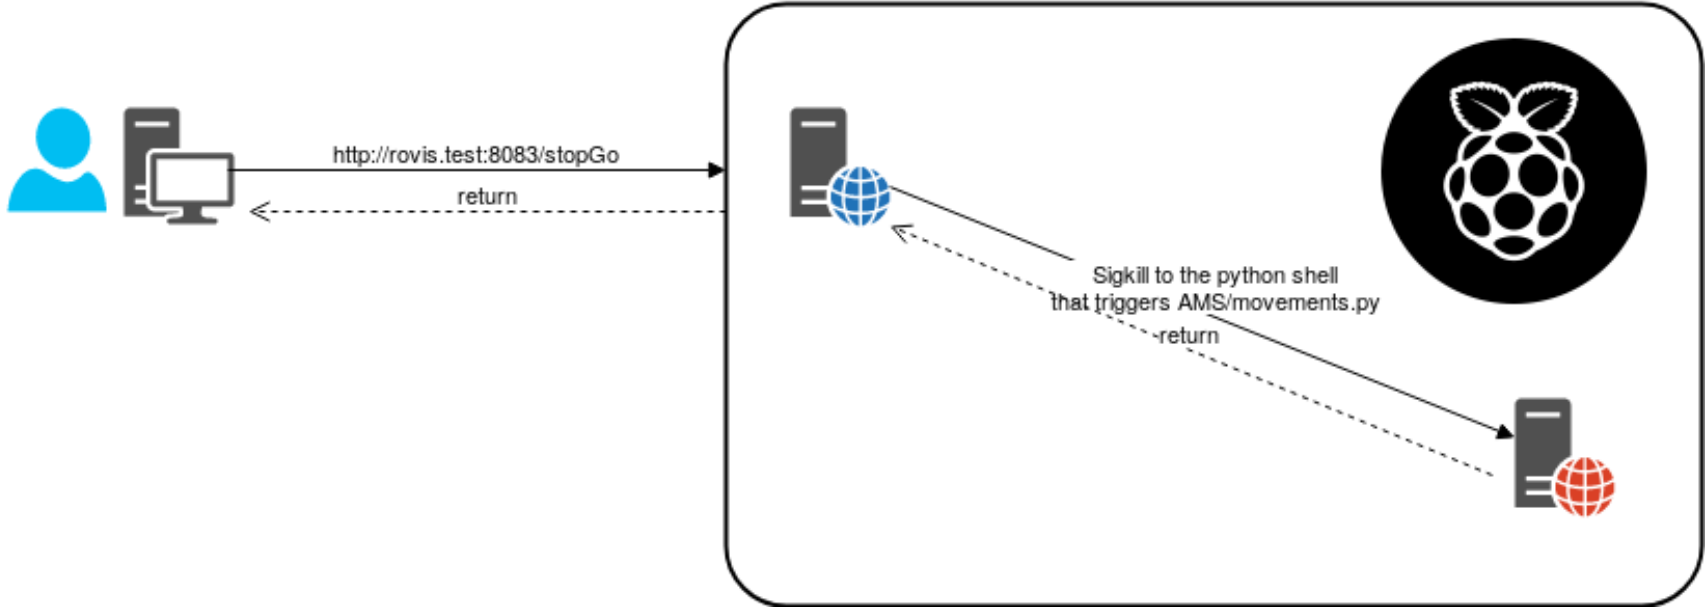
\includegraphics[width=\textwidth]{images/api4.png}
		\caption{Caso d'uso 4: \textbf{\textit{stop go}}}
		\label{fig:usecase4}
	\end{subfigure}
\end{figure}
\section{Realizzazione}
\subsection{Hardware} 
\subsection{Software}
Per garantire il controllo del dispositivo tramite un'interfaccia web è stato necessario progettare un server al quale un client può collegarsi per ottenere il controllo del dispositivo. È stato utilizzato il framework javascript \textit{NodeJs} per gestire sia la parte client che server dell'applicazione. Nelle seguenti sezioni verrà descritta la struttura gerarchica delle cartelle e le funzionalità presenti nei file al loro interno.
\paragraph{Server}
I file presenti all'interno della cartella \textit{server} contengono le funzioni per gestire la parte server del sistema, mentre all'interno delle sue sottocartelle sono presenti altri file che verranno descritti in seguito.\\
\paragraph{main.js}
Il file \textit{main.js} è il file principale del server. Al suo interno sono presenti le funzioni di inizializzazione del sistema e per la gestione dello streaming video.\\
Per avviare il server è necessario digitare il seguente comando:
\begin{lstinputlisting}[caption={Avvio server},basicstyle=\tiny]{codice/startServer}\end{lstinputlisting}
\begin{itemize}
	\item \textbf{node} nodejs;
	\item \textbf{main.js} file del server;
	\item \textbf{ciao} parola chiave; \todo{cambiare ciao}
	\item \textbf{8081 8082 8083}  qualcosa \todo{scrivere}
\end{itemize}
Una volta lanciato il comando, sarà possibile accedere all'interfaccia web digitando l'indirizzo IP del raspberry seguito da \textit{:8083}.
\begin{lstinputlisting}[caption={Esempio indirizzo server},basicstyle=\tiny]{codice/indirizzo}\end{lstinputlisting}
\paragraph{routes.js}
Questo file è quello che gestisce la comunicazione client server, associando ad ogni interazione del client sulla pagina web una specifica azione del server. Gestisce quindi le funzioni che regolano la webcam e il movimento. In particolare viene utilizzata una libreria di nodejs per eseguire la libreria Python \textit{AMSpi} per la gestione dei motori.
\paragraph{AMSpi}
\textit{AMSpi} è la libreria Python utilizzata per controllare i motori. Al suo interno è presente il file \textit{movements.py}. È il file che usa le funzioni della libreria per controllare i motori.
\paragraph{Client}
I file presenti all'interno della cartella \textit{public} sono quelli che gestiscono la parte client dell'applicazione.\\
\paragraph{ex3-1.html} 
\todo{immagine}
È il file contenente la struttura del sito web.
\paragraph{css}
All'interno di questa cartella sono presenti i file che regolano lo stile della pagina.
\paragraph{js}
In questa cartella sono contenuti i file che regolano le interazioni dell'utente con la pagina e comunicano al server le azioni intraprese da esso.

\section{Ulteriori sviluppi e Conclusioni}	
%\newpage	
%\bibliographystyle{abbrv}
%\bibliography{Bib}
\end{document}